\section{A test function for the band}\label{sec:test}

\subsection{The functions $\rho$ and $W$}

Let
\[
\rho(z)=\Big(\frac{z-a}{z-b}\Big)^{1/2}\Big(\frac{z+a}{z+b}\Big)^{1/2},
\qquad z\in\Cp,
\]
with principal square roots. The map $z\mapsto(z-a)/(z-b)$ is a real
M\"obius transformation of determinant $a-b<0$ and sends $\Cp$ onto the lower
half-plane; $z\mapsto(z+a)/(z+b)$ has determinant $b-a>0$ and sends $\Cp$ onto
itself. Neither meets the negative real axis, so $\rho$ is analytic and
zero-free in $\Cp$.\footnote{The principal square root is analytic and zero-free on $\C\setminus(-\infty,0]$, and an open half-plane bounded by the real axis does not meet $(-\infty,0]$.} Put
\begin{equation}\label{eq:W}
W(z)=\rho(z)-2+\frac1{\rho(z)}=\frac{(\rho(z)-1)^2}{\rho(z)} ,
\end{equation}
and, for $a<t<b$,
\begin{equation}\label{eq:p}
\begin{gathered}
r(t)=\sqrt{(t^2-a^2)(b^2-t^2)},\\
p(t)=\frac{a^2+b^2-2t^2}{r(t)}
=\sqrt{\frac{b^2-t^2}{t^2-a^2}}-\sqrt{\frac{t^2-a^2}{b^2-t^2}} .
\end{gathered}
\end{equation}

\begin{lemma}\label{lem:W}
\begin{enumerate}
\item[(i)] $\rho(-\bar z)=\overline{\rho(z)}$, and
$\rho(z)=1+\frac{b^2-a^2}{2z^2}+O(z^{-4})$, so $W(z)=O(z^{-4})$ as
$z\to\infty$ in $\overline{\Cp}$.
\item[(ii)] $\rho$ and $W$ extend continuously to $\overline{\Cp}$ minus the
four points $\pm a,\pm b$, near which $\abs{W(z)}=O(\abs{z\mp a}^{-1/2})$,
$O(\abs{z\mp b}^{-1/2})$.
\item[(iii)] On $\R\setminus S$, $\rho$ is real and positive, and
$W=(\rho-1)^2/\rho$ is real and strictly positive.
\item[(iv)] For $a<t<b$, $\rho(t+i0)=-i\,s(t)$ with
$s(t)=\sqrt{(t^2-a^2)/(b^2-t^2)}$, hence
\[
W(t)=-2+i\,p(t),\qquad W(-t)=-2-i\,p(t).
\]
\end{enumerate}
\end{lemma}

\begin{proof}
(i) The symmetry holds for each factor. Since
$\rho^2=(z^2-a^2)/(z^2-b^2)=1+(b^2-a^2)/(z^2-b^2)$ and $\rho\to1$, the
expansion follows, and $W=(\rho-1)^2/\rho$.
(ii) Near $b$ the factor $(z-a)/(z-b)$ behaves like a constant over $z-b$,
so $\rho\sim c(z-b)^{-1/2}$ and $W\sim\rho$; near $a$, $\rho\sim c(z-a)^{1/2}$ and
$W\sim1/\rho$. The points $-a,-b$ follow by symmetry.
(iii) For real $t\notin S$ both quotients are positive.
(iv) For $a<t<b$ and $\varepsilon\downarrow0$ the number
$(t-a)/(t-b+i\varepsilon)$ has negative real part and negative imaginary
part, so its principal square root tends to $-i\sqrt{(t-a)/(b-t)}$, while
$\sqrt{(t+a)/(t+b)}$ is positive. Hence $\rho=-is$ and
$W=-is-2+i/s=-2+i(1/s-s)=-2+ip$. The value at $-t$ follows from (i).
\end{proof}

\Cref{fig:testfunction} shows $\Re W$: a plateau at $-2$ over the band,
positive values elsewhere, and integrable spikes at the band edges.

\begin{figure}[t]
\centering
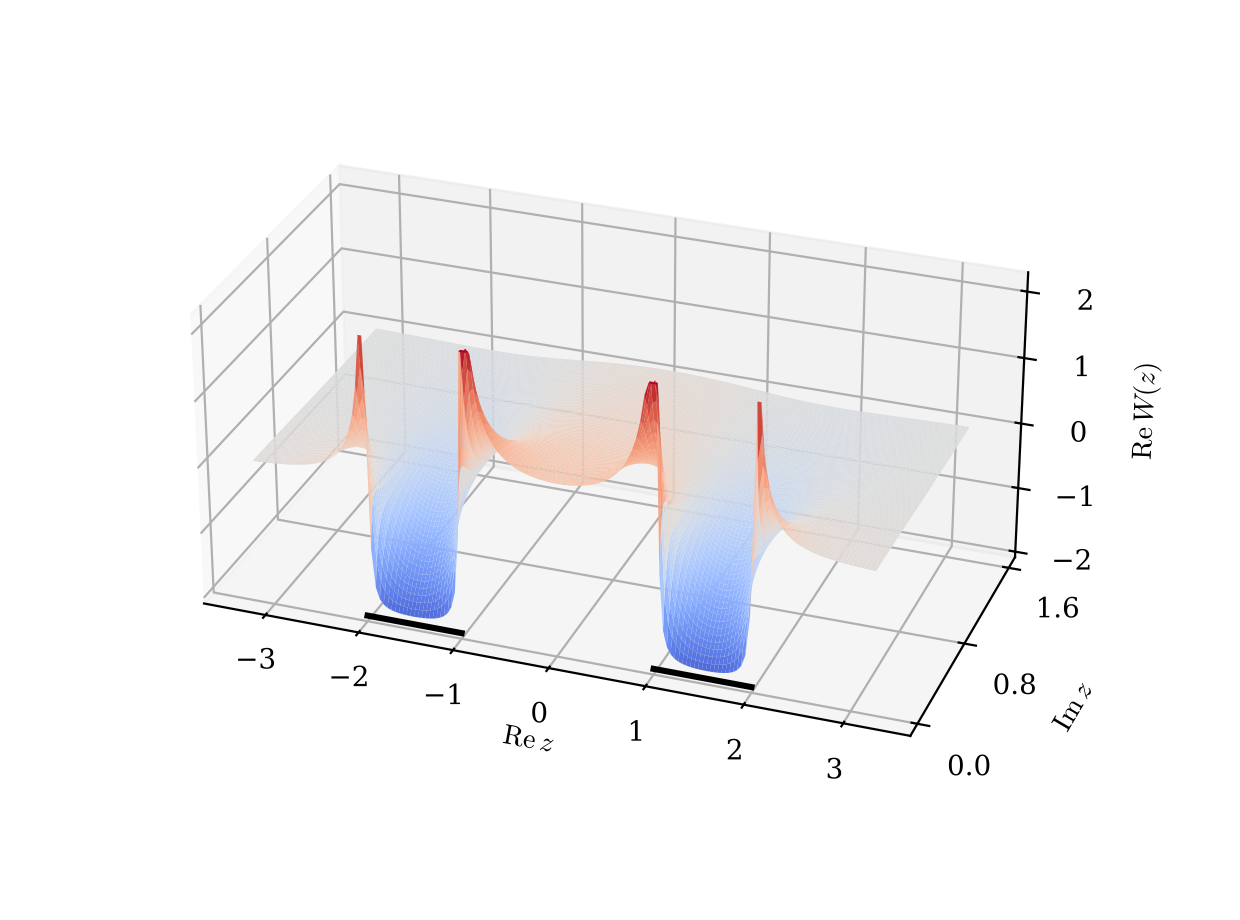
\includegraphics[width=\columnwidth]{figures/fig_testfunction.png}
\caption{The real part of the test function $W$ over the upper half-plane
for $a=1$, $b=2$ (values clipped at $\pm2.2$). On the real axis it equals $-2$
on the band (black segments) and is strictly positive elsewhere.}
\label{fig:testfunction}
\end{figure}

\subsection{The kernel identity}

\begin{lemma}\label{lem:kernel}
For $s>0$, $s\ne a,b$,
\begin{equation}\label{eq:kernel}
\frac1\pi\PV\int_a^b p(x)\,\frac{2x}{x^2-s^2}\dd x=
\begin{cases}-2,& a<s<b,\\ W(s),& s\notin[a,b].\end{cases}
\end{equation}
\end{lemma}

\begin{proof}
Apply Cauchy's theorem to $W(z)/(z-s)$ on the boundary of the half-disc of
radius $R$ in $\Cp$, indented by semicircles of radius $\varepsilon$ above
$s,\pm a,\pm b$. By \cref{lem:W}(ii) the small semicircles at $\pm a,\pm b$
contribute $O(\varepsilon^{1/2})$; by \cref{lem:W}(i) the large one
contributes $O(R^{-4})$; the one at $s$ contributes $-\pi iW(s)$ in the
limit, $W$ being continuous at $s$. Therefore
\[
\PV\int_\R\frac{W(x)}{x-s}\dd x=\pi i\,W(s).
\]
Taking imaginary parts and using that $\Im W$ vanishes off $S$ and equals
$\pm p(\abs x)$ on $\pm[a,b]$ (\cref{lem:W}(iii),(iv)),
\begin{align*}
\pi\Re W(s)&=\PV\int_a^bp(x)\Big(\frac1{x-s}+\frac1{x+s}\Big)\dd x\\
&=\PV\int_a^bp(x)\frac{2x}{x^2-s^2}\dd x .
\end{align*}
By \cref{lem:W}, $\Re W(s)=-2$ for $a<s<b$ and $\Re W(s)=W(s)$ otherwise.
\end{proof}

\begin{figure}[t]
\centering
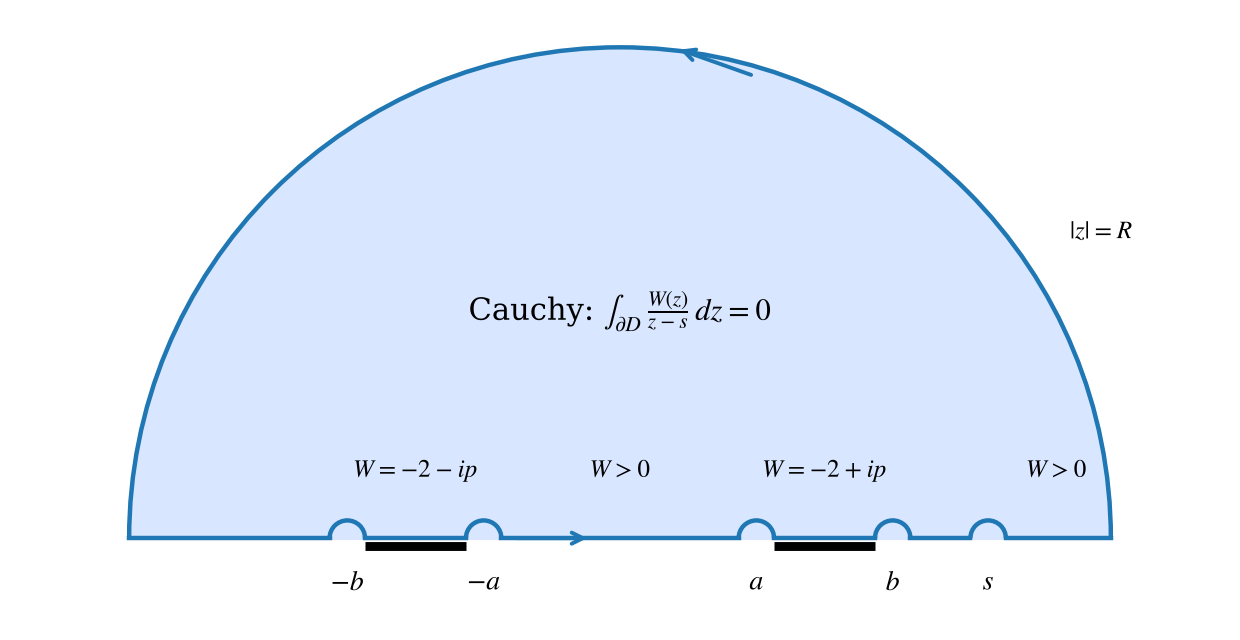
\includegraphics[width=\columnwidth]{figures/fig_contour.png}
\caption{The contour of the proof of \cref{lem:kernel}: a half-disc of
radius $R$ in $\Cp$, indented above the branch points $\pm a,\pm b$ of $W$
and above the pole $s$. The branch cuts of $W$ are the two bands $\pm[a,b]$
(thick); the indentations at the branch points contribute nothing in the
limit, the one at $s$ contributes $-\pi iW(s)$.}
\label{fig:contour}
\end{figure}

\subsection{Moments of the weight}

The weight $p$ is positive on $(a,c)$ and negative on $(c,b)$, where
$c^2=(a^2+b^2)/2$. Under $\sigma=x^2$ it becomes antisymmetric, and this
gives all the sign information we need.

\begin{lemma}\label{lem:moments}
Let $A=a^2$, $B=b^2$ and
$\varpi(\sigma)=(A+B-2\sigma)/\sqrt{(\sigma-A)(B-\sigma)}$, so that
$x\,p(x)\dd x=\frac12\varpi(x^2)\dd(x^2)$.
\begin{enumerate}
\item[(i)] $\varpi(A+B-\sigma)=-\varpi(\sigma)$, and $\int_a^bx\,p(x)\dd x=0$.
\item[(ii)] If $f$ is continuous and nonincreasing on $[A,B]$, then
$\int_a^bx\,p(x)f(x^2)\dd x\ge0$, with equality only for constant $f$.
\item[(iii)] $J:=\int_a^bp(x)\dd x>0$ and $\int_a^b\frac{p(x)}{x}\dd x
=\frac{\pi(b-a)^2}{2ab}$.
\item[(iv)] $\int_a^bx^{2j+1}p(x)\dd x<0$ for $j\ge1$, and
$\int_a^bx^3p(x)\dd x=-\frac\pi8(b^2-a^2)^2$.
\end{enumerate}
\end{lemma}

\begin{proof}
(i) The antisymmetry is visible, and it gives $\int_A^B\varpi=0$.
(ii) With $\sigma_m=(A+B)/2$,
\[
\int_a^bxpf(x^2)\dd x=\frac12\int_A^{\sigma_m}\varpi(\sigma)
\big(f(\sigma)-f(A+B-\sigma)\big)\dd\sigma ,
\]
and both factors are nonnegative for $\sigma<\sigma_m$; the integral vanishes
only if $f(\sigma)=f(A+B-\sigma)$ throughout, which for a monotone $f$ means
$f$ constant.
(iii) Apply (ii) to $f(\sigma)=\sigma^{-1/2}$ and $f(\sigma)=\sigma^{-1}$. The
value follows from the elementary integrals
\begin{gather*}
\int_A^B\frac{\dd\sigma}{\sqrt{(\sigma-A)(B-\sigma)}}=\pi,\\
\int_A^B\frac{\dd\sigma}{\sigma\sqrt{(\sigma-A)(B-\sigma)}}=\frac{\pi}{\sqrt{AB}},
\end{gather*}
which give $\frac12\big((A+B)\pi/\sqrt{AB}-2\pi\big)=\pi(b-a)^2/(2ab)$.
(iv) Apply (ii) to $f(\sigma)=-\sigma^j$. For $j=1$ use also
$\int_A^B\sigma\,\dd\sigma/\sqrt{\cdot}=\pi(A+B)/2$ and
$\int_A^B\sigma^2\dd\sigma/\sqrt\cdot=\pi(3A^2+2AB+3B^2)/8$.
\end{proof}

The first moment vanishing is the reason why delays are free; the positivity
of $J$ is the reason why a constant phase lag is not.
